%NYU 2019 Grad Computational Physics Homework 1

\documentclass[12pt, graphicx]{article}
\pagestyle{plain}
\baselineskip 18pt
\textwidth 6.5in
\textheight 7.8in
\oddsidemargin 0.1in
\evensidemargin 0.1in
\topmargin 0.3in
\parindent 0pt
\linespread{1.5}
\setlength{\parskip}{2.5mm}

\usepackage{graphicx, psfrag, epsfig}
\usepackage[font = small, format = plain, labelfont = bf, textfont = it, justification = raggedright, singlelinecheck = false]{caption}
\usepackage{subfig}
\usepackage{amsmath, amssymb}
\usepackage{geometry}
%\usepackage[symbol]{footmisc}

\renewcommand\tablename{Table}
\renewcommand\figurename{Fig.}
\renewcommand{\thefootnote}{\fnsymbol{footnote}}


\begin{document}
\title{Computational Physics Homework 1}
\author{Hao Li\footnotemark[2]}
\footnotetext[2]{hl3270@nyu.edu~~UID:N12137527}
\date{\today}


\maketitle

\section*{Problem 1}
\subsection*{a)}
The code for differentiating one-dimensional functions using single precision forward-, central-, and extrapolated-difference algorithms is available in \textquotedblleft differentiation\_1D.h\textquotedblright, attached in the folder.\par

This code returns the derivative with the least relative error, and save the step sizes $h$, the derivatives $f'(x)$, the absolute total errors $\mathrm{e}$, as well as the relative errors $\epsilon$ of every loop in a file. By chosing some pre-recorded functions (presently unable to enter functions from the commander line), of which the code is in \textquotedblleft function\_input.h\textquotedblright, and enter from the commander line the position $x$, the initial step size $h_0$, the user definded relative error tolerance $\epsilon_\mathrm{tol}$, and the maximum of loops $\mathrm{max\_loop}$ of calculatation, the calculation will continue until reaching the error tolerance or the maximum loop. \par

In this problem, since we want to see the relationship of relative error $\epsilon$ vs. step size $h$, a medium initial step size $h_0=0.5$, an unachivable error tolerance $\epsilon_\mathrm{tol}=1\mathrm{e}-8=1\times10^{-8}$, and a $\mathrm{max\_loop}=20$ were chosen. But in practice, $\epsilon$ may sometimes go to zero accidentally and thus end the calculation, so to get the whole $\log(\epsilon)-\log(h)$ plot, the break procedure was temporarily omitted.

\subsection*{b)}
The log-log plots of relative error $\epsilon$ vs. step size $h$ of the derivatives of $\cos(x)$ and $\mathrm{e}^x$ at $x=0.1,10$ in the three methods are shown below in Figure \ref{fig:dif_0.1} and \ref{fig:dif_10} respectively.

\begin{figure}[ht]
\begin{minipage}{0.48\linewidth}
\centering
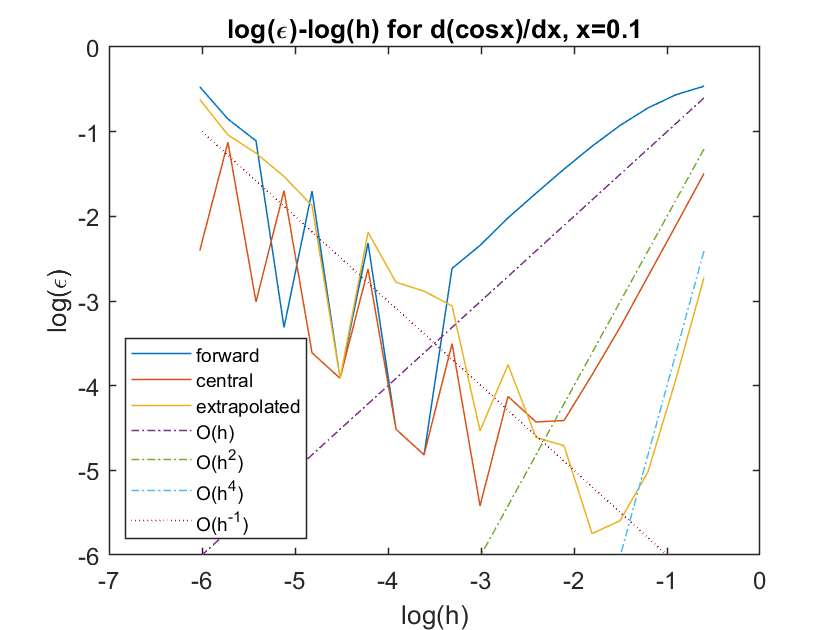
\includegraphics[width = 80mm]{dif_cos_1e-1.png}
\end{minipage}
\begin{minipage}{0.48\linewidth}
\centering
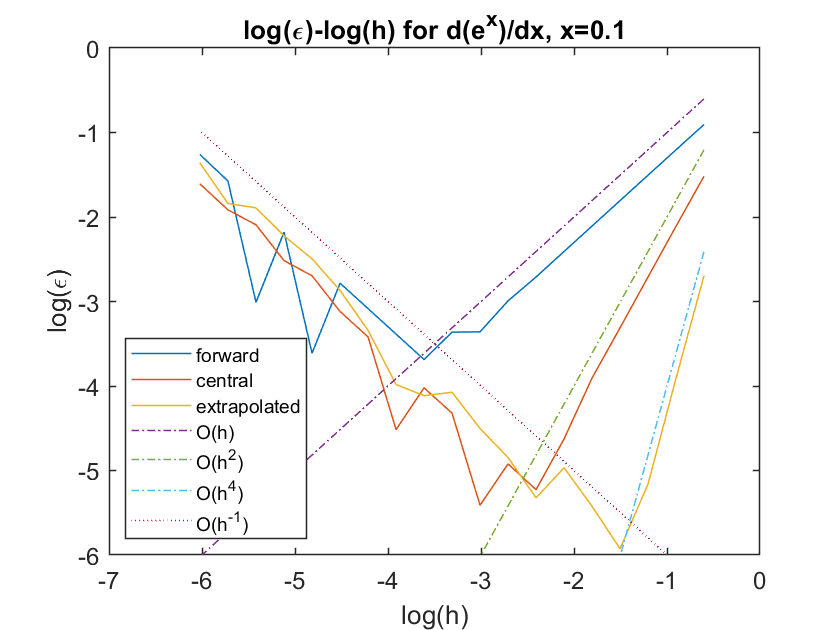
\includegraphics[width = 80mm]{dif_exp_1e-1.png}
\end{minipage}
\caption{$\log(\epsilon)-\log(h)$ plots of $\frac{\mathrm{d}\cos(x)}{\mathrm{d}x}|_{x=0.1}$ and $\frac{\mathrm{d}\mathrm{e}^x}{\mathrm{d}x}|_{x=0.1}$. Initial step size $h_0=0.5$, calculate for $\mathrm{max\_loop}=20$. $\epsilon_\mathrm{tol}=1\mathrm{e}-8$, but the code was set not to break to see the whole behavior. In these two plots, the error tolerence was not reached, as estimated.}
\label{fig:dif_0.1}
\end{figure}

\begin{figure}[ht]
\begin{minipage}{0.48\linewidth}
\centering
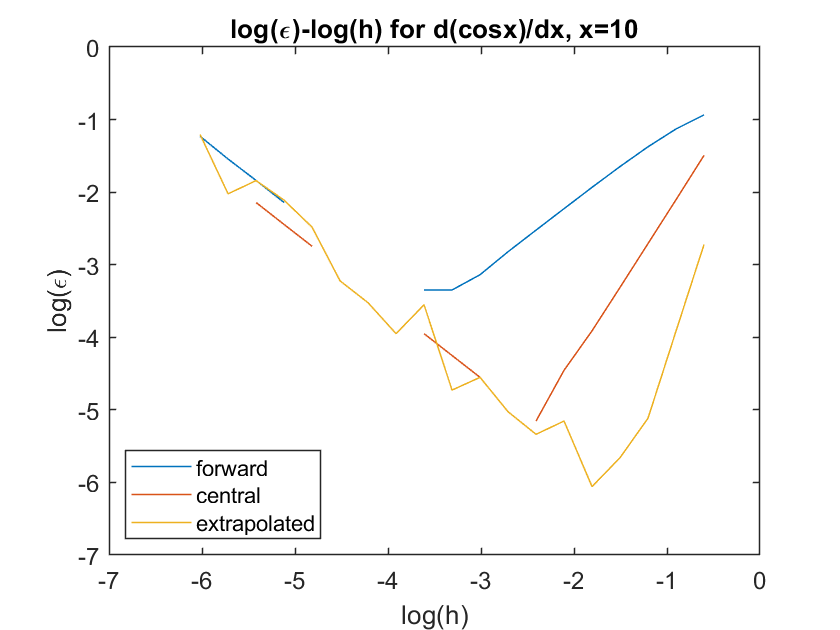
\includegraphics[width = 80mm]{dif_cos_10.png}
\end{minipage}
\begin{minipage}{0.48\linewidth}
\centering
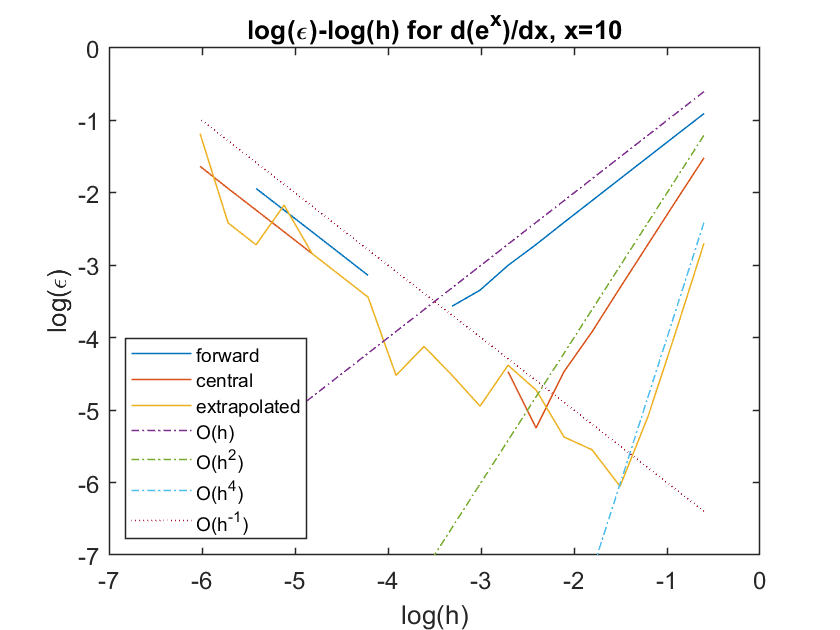
\includegraphics[width = 80mm]{dif_exp_10.png}
\end{minipage}
\caption{$\log(\epsilon)-\log(h)$ plots of $\frac{\mathrm{d}\cos(x)}{\mathrm{d}x}|_{x=10}$ and $\frac{\mathrm{d}\mathrm{e}^x}{\mathrm{d}x}|_{x=10}$. Initial step size $h_0=0.5$, calculate for $\mathrm{max\_loop}=20$. $\epsilon_\mathrm{tol}=1\mathrm{e}-8$, but the code was set not to break to see the whole behavior. However, the tolerence was reached accidentally when some $\epsilon$ goes to zero, which correspond to the points missing in the plots.}
\label{fig:dif_10}
\end{figure}

Initial step size is chosen to be $h_0=0.5$, calculate for $\mathrm{max\_loop}=20$, relative error tolerance $\epsilon_\mathrm{tol}=1\mathrm{e}-8$, but the code was set not to break to see the whole behavior. In Figure \ref{fig:dif_10} of $x=10$ we can see that, for some step sizes, $\epsilon$ accidentally goes to zero, so those points are missing in the plots.\par

Figure \ref{fig:dif_0.1} and \ref{fig:dif_10} show that when step size $h$ decreases, before the relative error $\epsilon$ goes down to optimal value, $\epsilon\sim h, h^2, h^4$ for forward-, central-, and extrapolated-difference algorithms respectively, which satiesfy the theoretical estimates. Below $h_\mathrm{opt}$, $\mathrm{\epsilon_r}\sim \mathrm{\epsilon_m}h^{-1}$ is the leading error, as shown in the plots. Also, it agrees well with the theory that the best relative error for the three methods are $\epsilon_\mathrm{opt}\approx10^{-3.5}, 10^{-5}, 10^{-6}$ respectively, i.e. the number of significant digits obtained matches with the estimates.

\subsection*{c)}
As mentioned in b), truncation error $\epsilon_\mathrm{t}$ manifest itself in the regime $h>h_\mathrm{opt}$, and for round-off error $\epsilon_\mathrm{r}$ is in $h>h_\mathrm{opt}$. In the order of the three algorithms above, $h_\mathrm{opt}\sim \epsilon_\mathrm{m}^{1/2}, \epsilon_\mathrm{m}^{1/3}, \epsilon_\mathrm{m}^{1/5}$. Since for $\cos(x)$ and $\mathrm{e}^x$ at 0.1, 10, $\frac{f}{f''}\approx 1$, so $h_\mathrm{opt}\approx 10^{-3.5}, 10^{-2.5}, 10^{-1.5}$, for single precision(machine precision $\epsilon_\mathrm{m}\approx 10^{-7}$).


\section*{Problem 2}
\subsection*{a)}
The code for integrating one-dimensional functions using single precision midpoint, trapezoid, and Simpson's rule is available in \textquotedblleft integration\_1D.h\textquotedblright, attached in the folder.\par

This code returns the integral with the least relative error, and save the number of bins $N$, the integrals $\int_a^bf(x)\mathrm{d}x$, the absolute total errors $\mathrm{e}$, as well as the relative errors $\epsilon$ of every loop in a file. By chosing some pre-recorded functions (presently unable to enter functions from the commander line), of which the code is in \textquotedblleft function\_input.h\textquotedblright, and enter from the commander line the lower and the upper bounds $a,b$, the initial number of bins $N_0$, the user definded relative error tolerance $\epsilon_\mathrm{tol}$, and the maximum of loops $\mathrm{max\_loop}$ of calculatation, the calculation will continue until reaching the error tolerance or the maximum loop. \par

In this problem, since we want to see the relationship of relative error $\epsilon$ vs. number of bins $N$, a medium initial number of bins $N_0=2$, an unachivable error tolerance $\epsilon_\mathrm{tol}=1\mathrm{e}-8=1\times10^{-8}$, and a $\mathrm{max\_loop}=20$ were chosen. But in practice, $\epsilon$ may sometimes go to zero accidentally and thus end the calculation, so to get the whole $\log(\epsilon)-\log(h)$ plot, the break procedure was temporarily omitted.

\subsection*{b)}
The log-log plots of relative error $\epsilon$ vs. number of bins $N$ of $\int_0^1\mathrm{e}^{-t}\mathrm{d}t$ in the three methods are shown in Figure \ref{fig:int_exp_10}.

\begin{figure}[ht]
\centering
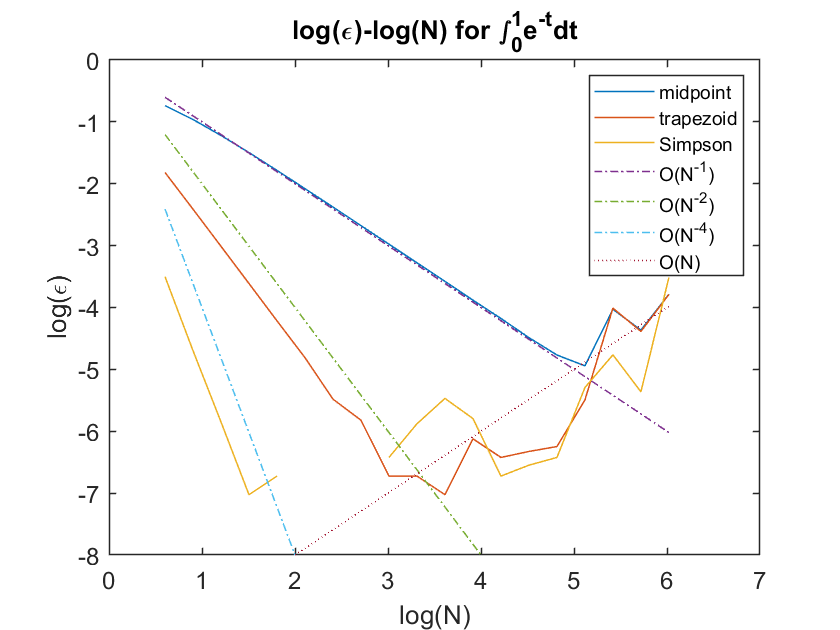
\includegraphics[width = 120mm]{int_exp-x.png}
\caption{$\log(\epsilon)-\log(N)$ plots of $\int_0^1\mathrm{e}^{-t}\mathrm{d}t$. Initial number of bins $N_0=2$, calculate for $\mathrm{max\_loop}=20$. $\epsilon_\mathrm{tol}=1\mathrm{e}-8$, but the code was set not to break to see the whole behavior. However, the tolerence was reached accidentally when some $\epsilon$ goes to zero, which correspond to the points missing in the plots.}
\label{fig:int_exp_10}
\end{figure}

Initial number of bins is chosen to be $N_0=2$, calculate for $\mathrm{max\_loop}=20$, relative error tolerance $\epsilon_\mathrm{tol}=1\mathrm{e}-8$, but the code was set not to break to see the whole behavior. In Figure \ref{fig:int_exp_10} we can see that, for some $N$'s for Simpson's rule, $\epsilon$ accidentally goes to zero, so those points are missing in the plots.\par

\subsection*{c)}
Figure \ref{fig:int_exp_10} shows that when number of bins $N$ decreases, before the relative error $\epsilon$ goes down to optimal value, $N<N_\mathrm{opt}$, truncation error $\epsilon_\mathrm{t}$ manifest itself in the regime, so $\epsilon\sim N, N^{-2}, N^{-4}$ for midpoint, trapezoid, and Simpson's rules respectively, which satiesfy the theoretical estimates. Above $N_\mathrm{opt}$, round-off error is the leading error, as shown in the figures. Similar to differentiation, the optimal number of bins $N_\mathrm{opt}\mathrm{(midpoint)}>N_\mathrm{opt}\mathrm{(trapezoid)}>N_\mathrm{opt}\mathrm{(Simpson's)}$, and the best relative error $\epsilon_\mathrm{opt}\mathrm{(midpoint)}<\epsilon_\mathrm{opt}\mathrm{(trapezoid)}<\epsilon_\mathrm{opt}\mathrm{(Simpson's)}$, as estimated.


\section*{Problem 3}
The plot and the log-log plot of the power spectrum $P(k)$ are shown in Figure \ref{fig:Pk}. In the log-log plot, we can clearly see a \textquotedblleft baryon wiggle" within $k\in[10^{-1}, 10^{-2}]$.

\begin{figure}[ht]
\begin{minipage}{0.48\linewidth}
\centering
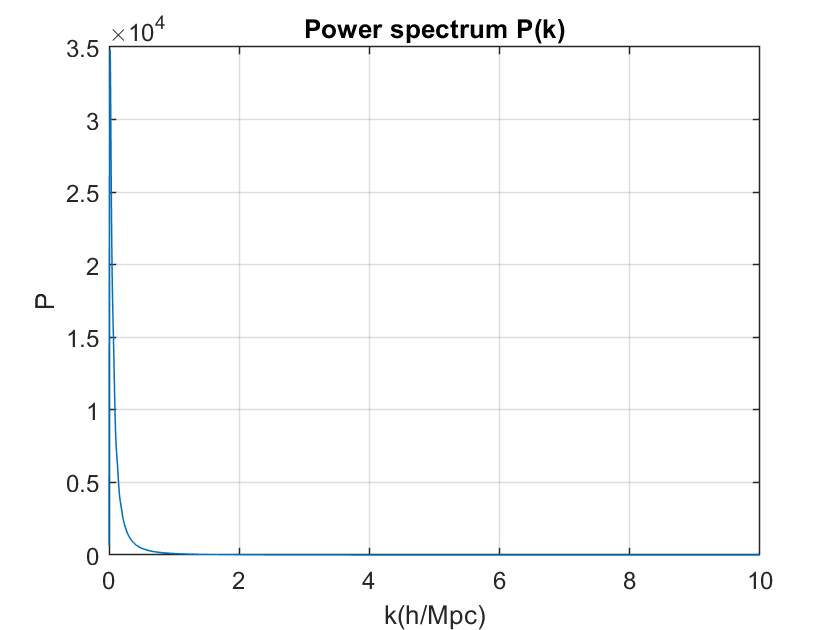
\includegraphics[width = 80mm]{Pk.png}
\end{minipage}
\begin{minipage}{0.48\linewidth}
\centering
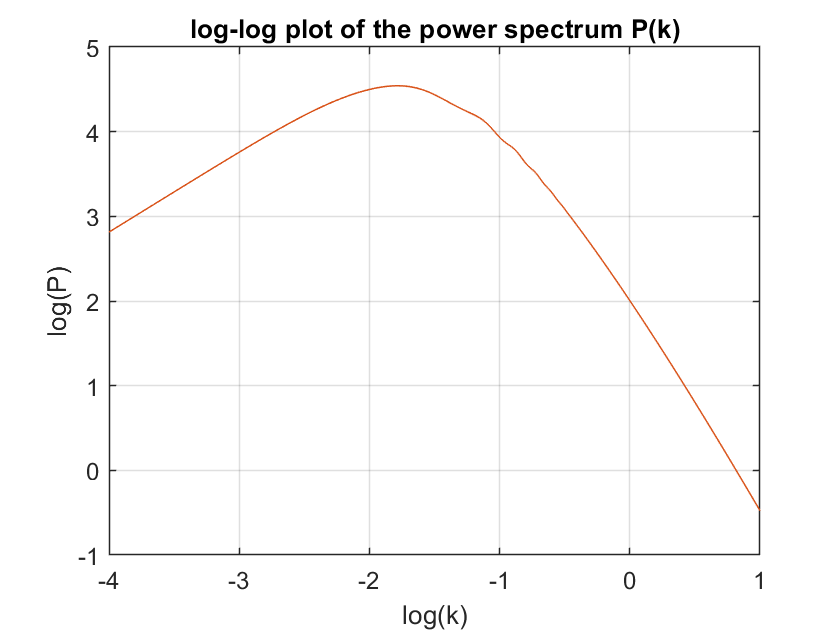
\includegraphics[width = 80mm]{logPk.png}
\end{minipage}
\caption{The plot and the log-log plot of the power spectrum $P(k)$}
\label{fig:Pk}
\end{figure}

According to the notes, $\displaystyle\lim_{k\to0}P(k)=\lim_{k\to+\infty}P(k)=0$. As a good approximation for the whole power spectrum within $k\in[0,+\infty)$, the log-log plots of $P(k)$ for $[0,k_0]$ and $[k_N, +\infty]$ are linear, where $N$ is the number of data points in the file (in this problem is 501), and $k_0,k_N$ are the minimum and maximum wave number in the data. The slopes of the two lines are the same as the derivative of the cubic spline of $\log(P)-\log(k)$ at $k_0,k_N$. \par

From the cubic spline result of the $P(k)$ data in the data file provided, we estimate that 
\begin{equation}
P(k)|_{k\in[0,10^{-4}]}=P(k=10^{-4})\cdot(\frac{k}{10^{-4}})^{f'_0}=651.34\cdot(\frac{k}{10^{-4}})^{0.94963}
\end{equation}
\begin{equation}
P(k)|_{k\in[10,+\infty]}=P(k=10)\cdot(\frac{k}{10})^{f'_N}=0.33403\cdot(\frac{k}{10})^{-2.6189}
\end{equation}
which satiesfy the boundary condition of the power spectrum. In the data range $[k_0,k_N]$, since the power spectrum is tabulated in logarithmic intervals, assume $x=\log k$, in each interval $x\in[x_i, x_{i+1}]=[\log k_i,\log k_{i+1}]$, 
\begin{equation}
P(x)|_{x\in[x_i,x_{i+1}]}=P(x_i)\cdot10^{a_i(x-x_i)^3+b_i(x-x_i)^2+c_i(x-x_i)}
\end{equation}
here $a_i,b_i,c_i$ are the coefficients of the cubic spline result of the log-log plot of the power spectrum in the i'th bin $[k_i,k_{i+1}]$
\begin{equation}
\log P(k)|_{k\in[k_i,k_{i+1}]}-\log P(k_i)=a_i(\log k-\log k_i)^3+b_i(\log k-\log k_i)^2+c_i(\log k-\log k_i)
\end{equation}
Now that we have the whole expression of the power spectrum, we can calculate the integral of correlation function in bins.\par 

(1) For $k<k_\mathrm{min}=10^{-4}$, we directly use the given expression 
\begin{equation}
\xi_1(r)=\frac{1}{2\pi^2}\int_0^{10^{-4}}\mathrm{d}k\cdot k^2P(k)\frac{\sin(kr)}{kr}
\end{equation}
using Romberg integration for faster speed. The result of this part
\begin{equation}
\xi_1(r)\approx 8.3547\times 10^{-12}
\end{equation}
is quite small relative to the whole integral $\xi(r)>10^{-4}$ and hardly varies. \par

(2) For within data range $k\in[k_\mathrm{min},k_\mathrm{min}]=[10^{-4},10]$, we change the independent variable from $k$ to $x=\log(k)$, new expression 
\begin{equation}
\xi_2(r)=\frac{\ln 10}{2\pi^2r}\int_{10^{-4}}^{10}\mathrm{d}x\cdot 10^{2x}P(x)\sin(r\cdot 10^x)=\frac{\ln 10}{2\pi^2r}\displaystyle\sum_{i=0}^{N-1}\int_{x_i}^{x_{i+1}}\mathrm{d}x\cdot 10^{2x}P(x)\sin(r\cdot 10^x)
\end{equation}
Calculate the integral of each bin using Simpson's rule for stable result.\par

(3) For $k>k_\mathrm{max}=10$, we still use the direct expression
\begin{equation}
\xi_3(r)=\frac{1}{2\pi^2}\int_{10}^{+\infty}\mathrm{d}k\cdot k^2P(k)\frac{\sin(kr)}{kr}
\end{equation}
since although for integral over infinite range we can change variable, we will instead get another infinite value and highly oscillatory integral, which is even harder to calculate. Assume $y=1/k$, that expression is 
\begin{equation}
\xi_3(r)=\frac{1}{2\pi^2r}\int_0^{0.1}\mathrm{d}y\cdot \frac{1}{y^3}P(\frac{1}{y})\sin(\frac{r}{y})
\end{equation}
The integrated function is highly oscillatory and is not finite when $y\to 0$. Therefore, we instead use the origional expression and set a finite upper limit to get a good approximation of $\xi_3(r)$, since the integral converges. After testing for some $r\in[50,120]$ in Mathematica, 5000 is chosen to be the upper limit, for fairly good accuracy, fast speed and less error spikes. 

\begin{figure}[ht]
\begin{minipage}{0.48\linewidth}
\centering
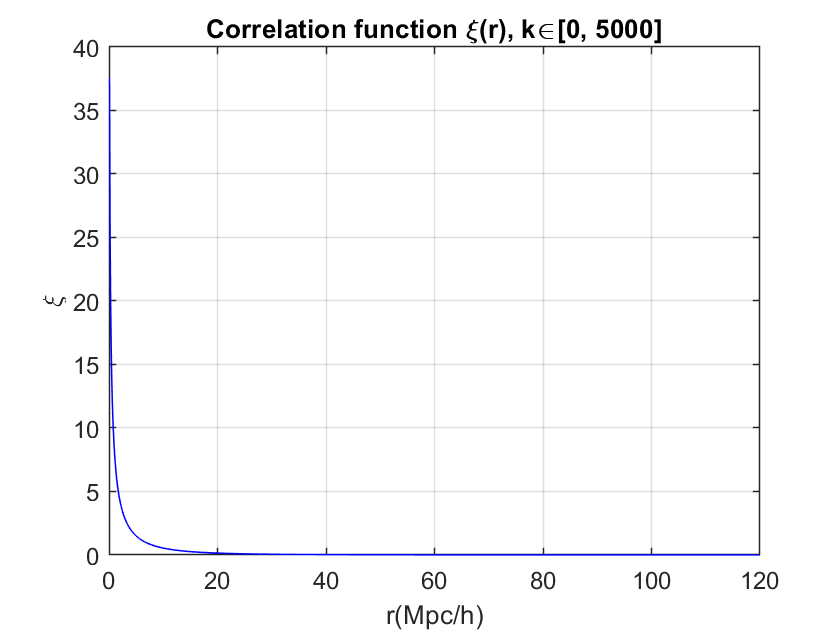
\includegraphics[width = 80mm]{xi_r_detailed.png}
\end{minipage}
\begin{minipage}{0.48\linewidth}
\centering
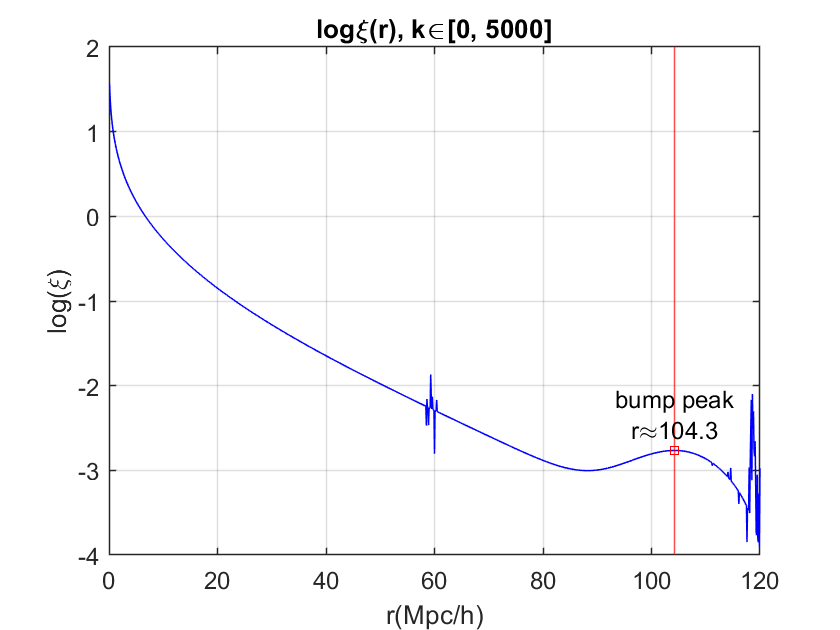
\includegraphics[width = 80mm]{logxi_r_detailed.png}
\end{minipage}
\caption{The plot of the correlation function $\xi(r)$ and $\log \xi(r)$. From the log plot we can see clearer the peak of the bump of $\xi(r)$}
\label{fig:xi}
\end{figure}

Figure \ref{fig:xi} is the plot of correlation function $\xi(r)$, integrated over $k\in[0,500]$. From the plot of $\log \xi(r)$, we can see a clear bump with peak at $r\approx104.3$. Also from this plot and the output datafile we can see that at arround $r=60,120$, there are some error spikes in the correlation function, entirely comming from $\xi_3(r)$, maybe because arround that scale, the error in each bin of the integral $\xi_3(r)$ tend to be of the same sign and accumulate to a large error, while when away from these scales the errors will cancel thus gives a smooth result.\par

\begin{figure}[ht]
\begin{minipage}{0.48\linewidth}
\centering
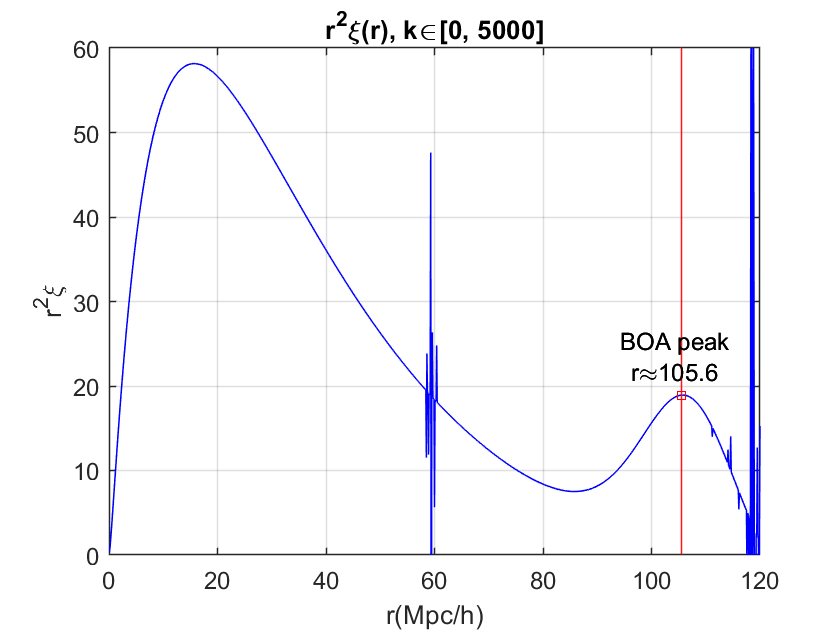
\includegraphics[width = 80mm]{r2xi_r_detailed.png}
\end{minipage}
\begin{minipage}{0.48\linewidth}
\centering
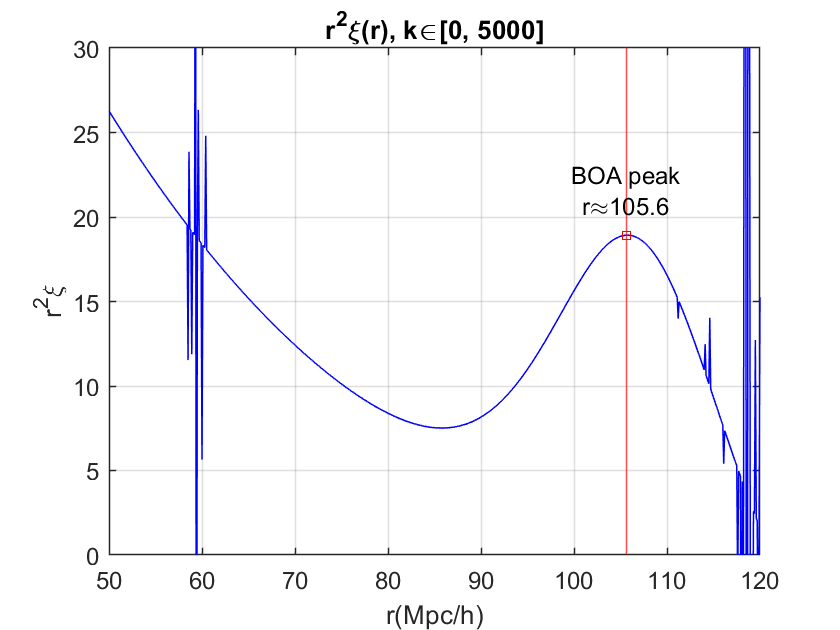
\includegraphics[width = 80mm]{r2xi_r_part_detailed.png}
\end{minipage}
\caption{The plot of $r^2\xi(r)$, where $\xi(r)$ is the correlation function. The \textquotedblleft baryon acoustic oscillation" (BOA) peak is at $r\approx105.6$. In this plot we can see clearly how much influence the small error spikes in $\xi_3(r)$ will have on the $r^2\xi(r)$ plot. However, since the upper limit of the integral was chosen to be big enough, so that the plot is still smooth enough in most $r$'s except those spikes.}
\label{fig:r2xi}
\end{figure}

Figure \ref{fig:r2xi} shows the plot of $r^2\xi(r)$ over $[0,120]$ and the required range $[50,120]$. Although it seems from the output datafile of $r^2\xi(r)$ that $\xi_3(r)$ is relatively small compared to $\xi_2(r)$, in Figure \ref{fig:r2xi2}, however, it is obvious that there are some small oscillations, while in Figure \ref{fig:r2xi} there are not. Therefore, $\xi_3(r)$ should not be omitted even it is small. 

\begin{figure}[ht]
\centering
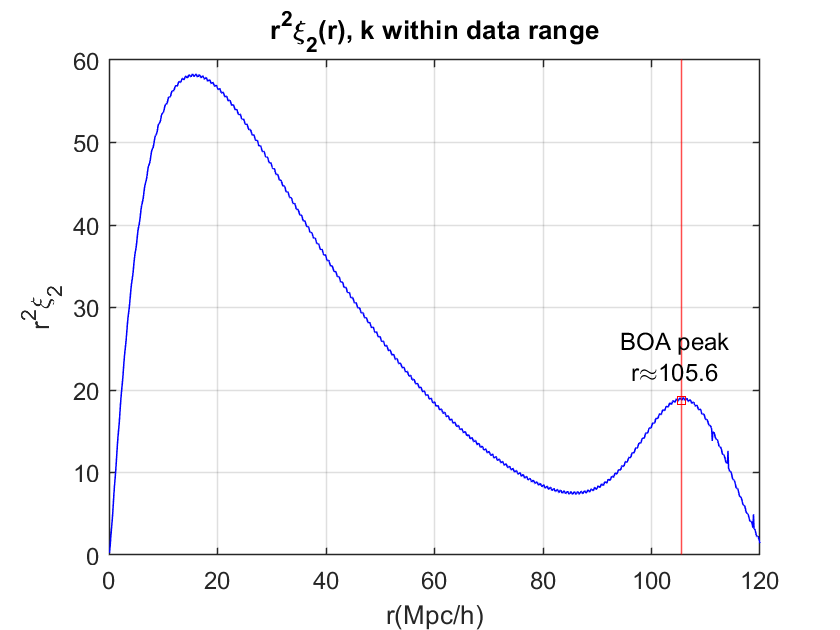
\includegraphics[width = 140mm]{r2xi2_r_detailed.png}
\caption{The plot of $r^2\xi_2(r)$, integrated only over the data range $[k_0,k_N]$. Small oscillations are clear and cannot be neglected, so the integrals below and over this range should be considered to get a smooth plot of $r^2\xi(r)$.}
\label{fig:r2xi2}
\end{figure}

According to Figure \ref{fig:r2xi}, the \textquotedblleft baryon acoustic oscillation" (BOA) peak is at arround the scale  $r=105.6\mathrm{(Mpc/h)}$.

\end{document}

